%% abtex2-modelo-relatorio-tecnico.tex, v-1.9.6 laurocesar
%% Copyright 2012-2016 by abnTeX2 group at http://www.abntex.net.br/ 
%%
%% This work may be distributed and/or modified under the
%% conditions of the LaTeX Project Public License, either version 1.3
%% of this license or (at your option) any later version.
%% The latest version of this license is in
%%   http://www.latex-project.org/lppl.txt
%% and version 1.3 or later is part of all distributions of LaTeX
%% version 2005/12/01 or later.
%%
%% This work has the LPPL maintenance status `maintained'.
%% 
%% The Current Maintainer of this work is the abnTeX2 team, led
%% by Lauro César Araujo. Further information are available on 
%% http://www.abntex.net.br/
%%
%% This work consists of the files abntex2-modelo-relatorio-tecnico.tex,
%% abntex2-modelo-include-comandos and abntex2-modelo-references.bib
%%

% ------------------------------------------------------------------------
% ------------------------------------------------------------------------
% abnTeX2: Modelo de Relatório Técnico/Acadêmico em conformidade com 
% ABNT NBR 10719:2015 Informação e documentação - Relatório técnico e/ou
% científico - Apresentação
% ------------------------------------------------------------------------ 
% ------------------------------------------------------------------------

\documentclass[
	% -- opções da classe memoir --
	12pt,				% tamanho da fonte
	openright,			% capítulos começam em pág ímpar (insere página vazia caso preciso)
	oneside,			% para impressão em recto e verso. Oposto a oneside
	a4paper,			% tamanho do papel. 
	% -- opções da classe abntex2 --
	%chapter=TITLE,		% títulos de capítulos convertidos em letras maiúsculas
	%section=TITLE,		% títulos de seções convertidos em letras maiúsculas
	%subsection=TITLE,	% títulos de subseções convertidos em letras maiúsculas
	%subsubsection=TITLE,% títulos de subsubseções convertidos em letras maiúsculas
	% -- opções do pacote babel --
	english,			% idioma adicional para hifenização
	french,				% idioma adicional para hifenização
	spanish,			% idioma adicional para hifenização
	brazil,				% o último idioma é o principal do documento
	]{abntex2}

% ---
% PACOTES
% ---

% ---
% Pacotes fundamentais 
% ---
\usepackage{lmodern}			% Usa a fonte Latin Modern
\usepackage[T1]{fontenc}		% Selecao de codigos de fonte.
\usepackage[utf8]{inputenc}		% Codificacao do documento (conversão automática dos acentos)
\usepackage{indentfirst}		% Indenta o primeiro parágrafo de cada seção.
\usepackage{color}				% Controle das cores
\usepackage{graphicx}			% Inclusão de gráficos
\usepackage{microtype} 			% para melhorias de justificação
\usepackage{array}
\usepackage{longtable}

\usepackage{tabularray}
\usepackage{rotating}
\usepackage{listings}
\usepackage{pdflscape} % mudar a orientação da página 
% ---

% ---
% Pacotes adicionais, usados no anexo do modelo de folha de identificação
% ---
\usepackage{multicol}
\usepackage{multirow}
% ---
	
% ---
% Pacotes adicionais, usados apenas no âmbito do Modelo Canônico do abnteX2
% ---
\usepackage{lipsum}				% para geração de dummy text
% ---

% ---
% Pacotes de citações
% ---
\usepackage[brazilian,hyperpageref]{backref}	 % Paginas com as citações na bibl
\usepackage[alf]{abntex2cite}	% Citações padrão ABNT

% --- 
% CONFIGURAÇÕES DE PACOTES
% --- 

% ---
% Configurações do pacote backref
% Usado sem a opção hyperpageref de backref
\renewcommand{\backrefpagesname}{Citado na(s) página(s):~}
% Texto padrão antes do número das páginas
\renewcommand{\backref}{}
% Define os textos da citação
\renewcommand*{\backrefalt}[4]{
	\ifcase #1 %
		Nenhuma citação no texto.%
	\or
		Citado na página #2.%
	\else
		Citado #1 vezes nas páginas #2.%
	\fi}%
% ---

% ---
% Informações de dados para CAPA e FOLHA DE ROSTO
% ---
\titulo{RELATÓRIO TÉCNICO: APLICATIVO DE CARONAS REGIONAL}

\autor{%
	Afrânio Martins Caires
	\\
	Daiane Rocha Teixeira
	\\
	Elizabeth Barbosa de Souza 
	\\
	João Eduardo Fernandes de Araújo
	\\
	Sávio Campos Vieira
	\\
	Vanderson Lopes Amaral 
}
\local{Araçuaí--MG}
\data{2024}
\instituicao{%
  Instituto Federal de Educação, Ciência e Tecnologia do Norte de Minas Gerais (IFNMG)
  \par
  Tecnologia em Análise e Desenvolvimento de Sistemas
  \par
  Núcleo de Informática}
\tipotrabalho{Relatório técnico}
% O preambulo deve conter o tipo do trabalho, o objetivo, 
% o nome da instituição e a área de concentração 
\preambulo{Relatório técnico para descrição da modelagem, codificação e demais atividades realizadas durante o Projeto Integrador em Análise e Desenvolvimento de Sistemas. Aplicativo de Caronas Regional: VemComigo}
% ---

% ---
% Configurações de aparência do PDF final

% alterando o aspecto da cor azul
\definecolor{blue}{RGB}{41,5,195}

% informações do PDF
\makeatletter
\hypersetup{
     	%pagebackref=true,
		pdftitle={\@title}, 
		pdfauthor={\@author},
    	pdfsubject={\imprimirpreambulo},
	    pdfcreator={LaTeX with abnTeX2},
		pdfkeywords={abnt}{latex}{abntex}{abntex2}{relatório técnico}, 
		colorlinks=true,       		% false: boxed links; true: colored links
    	linkcolor=black,          	% color of internal links
    	citecolor=black,        		% color of links to bibliography
    	filecolor=magenta,      		% color of file links
		urlcolor=blue,
		bookmarksdepth=4
}
\makeatother
% --- 

% --- 
% Espaçamentos entre linhas e parágrafos 
% --- 

% O tamanho do parágrafo é dado por:
\setlength{\parindent}{1.3cm}

% Controle do espaçamento entre um parágrafo e outro:
\setlength{\parskip}{0.2cm}  % tente também \onelineskip

% ---
% compila o indice
% ---
\makeindex
% ---


% ----------------------------------
% Definindo o template para o rodapé de continuação de tabela
\DefTblrTemplate{contfoot-text}{normal}{\centering \textit{Continuação da tabela \thetable\ na próxima página}}
\SetTblrTemplate{contfoot-text}{normal}

% Definindo o template para o cabeçalho de continuação de tabela
\DefTblrTemplate{conthead-text}{normal}{}
\SetTblrTemplate{conthead-text}{normal}
%--
%------------------------------------------------------------------

% ----
% Início do documento
% ----
\begin{document}

% Seleciona o idioma do documento (conforme pacotes do babel)
%\selectlanguage{english}
\selectlanguage{brazil}

% Retira espaço extra obsoleto entre as frases.
\frenchspacing 

% ----------------------------------------------------------
% ELEMENTOS PRÉ-TEXTUAIS
% ----------------------------------------------------------
% \pretextual

% ---
% Capa
% ---
\imprimircapa
% ---

% ---
% Folha de rosto
% (o * indica que haverá a ficha bibliográfica)
% ---
\imprimirfolhaderosto*
% ---

% ---
% LISTA DE ILUSTRAÇÕES
% ---
%\pdfbookmark[0]{\listfigurename}{lof}
%\listoffigures*
%\cleardoublepage
% ---

% ---
% LISTA DE TABELAS
% ---
%\pdfbookmark[0]{\listtablename}{lot}
%\listoftables*
%\cleardoublepage
% ---

% ---
% inserir o sumario
% ---
\pdfbookmark[0]{\contentsname}{toc}
\tableofcontents*
\cleardoublepage
% ---


% ----------------------------------------------------------
% ELEMENTOS TEXTUAIS
% ----------------------------------------------------------
\textual
% ---
% Introdução
% ---
\chapter{INTRODUÇÃO}

A mineração é uma atividade imprescindível para a manutenção e o desenvolvimento da sociedade. O ser humano está sempre buscando novas formas de facilitar a sua sobrevivência por meio de ferramentas criadas com os minérios extraídos da terra, que vão desde um simples livro, que necessita da celulose, um polímero extraído de fontes vegetais, até às grandes invenções como aviões e computadores.

Nota-se um aumento na demanda mundial por lítio, causado por uma corrida incessante para a substituição da atual matriz energética. O site Statista, plataforma global de dados e \textit{business intelligence}, registrou um salto crescente da demanda de tal mineral no mercado global entre os anos de 2022 e 2023, além de expectativas maiores para a próxima década, assim afirma \citeonline{demandaLitio} em sua publicação. No Brasil, uma região se destaca na oferta de jazidas minerais: o Vale do Jequitinhonha.

Paralelamente ao progresso, a mineração de lítio, no entanto, levanta questões complexas que envolvem aspectos ambientais, econômicos e sociais. Este capítulo tem a finalidade de apresentar um relatório técnico sobre o desenvolvimento de um software de caronas, criado com o objetivo de resolver uma das demandas atuais causadas pelo novo ciclo econômico da região.



\section{Contextualização}

O \textit{“Lithium Valley Brazil”} (Vale do Lítio Brasileiro) foi o nome dado ao novo projeto estadual de extrativismo em Minas Gerais. De acordo com o Governo do Estado de Minas Gerais, \citeonline{lancaValeDoLitio}, no dia 9 de maio, durante um evento da bolsa de valores em Nova Iorque, conhecida como \textit{Nasdaq} (\textit{National Association of Securities Dealers Automated Quotations}; em português, ``Associação Nacional de Corretores de Títulos de Cotações Automáticas''), o até então governador, Romeu Zema, liderou uma iniciativa responsável por atrair investidores do mundo inteiro. 

Mais uma vez, o Estado de Minas surpreendeu a indústria mundial com uma recente descoberta de ricas jazidas de lítio, mineral de suma importância para a economia global, sendo utilizado em ligas metálicas, medicamentos e, principalmente, nas baterias de celulares, computadores e carros elétricos. O lítio é extraído com a finalidade de ser exportado, assim como a maioria dos minérios.

Segundo a Secretaria de Desenvolvimento Econômico de Minas Gerais, \citeonline{EnviaLitio}, as primeiras 15 mil toneladas de lítio extraídas no Vale do Jequitinhonha foram entregues no Porto de Vitória, no Estado do Espírito Santo, em julho, assim sendo o pontapé inicial de um projeto audaz, coordenado pelo Governo de Minas Gerais, com a finalidade de atrair investimentos e empregos ao passo que promete desenvolver a região. A cobiça pelo ``Ouro Branco'', nome popular do mineral, está associada a uma demanda cada vez maior por fontes de energia limpa como alternativa aos combustíveis fósseis. O lítio se tornou responsável por intensas disputas geopolíticas pelo seu domínio uma vez que a Tesla, empresa norte-americana de carros elétricos gerenciada pelo bilionário Elon Musk, disputa com gigante chinesa BYD pela prioridade na compra do lítio extraído no Vale do Jequitinhonha, assim afirma \citeonline{agenciaBrasil}, repórter da Agência Brasil, em sua publicação.

Entre as empresas de mineração que operam na região em destaque encontra-se a \textit{Sigma Lithium}, empresa canadense que se destaca no cenário global de extração do lítio. No início de 2023, a empresa inaugurou o seu complexo, atualmente o quarto maior produtor mundial de acordo com a \citeonline{GrotadoCirilo}, um projeto de extração baseado na sustentabilidade. Toda a cadeia de produção não usará barragens de rejeito, água potável, agentes químicos nocivos ao ambiente ou carvão mineral como fonte de energia, assim batizando o seu produto final como Lítio Verde.

Entretanto, apesar das expectativas criadas ao redor de tal minério, nota-se alguns impactos na região brasileira mais promissora para a extração do lítio. Uma das demandas causadas pelo atual ciclo econômico surge do fato de que a região carece de estrutura urbana adequada. Em uma reportagem do Brasil de Fato MG, de \citeonline{BrasildeFatoProblemadaMineracao}, moradores apontam problemas como superlotação de equipamentos públicos de saúde, adoecimento mental e físico, contaminação das águas, danos nas estruturas das casas e desgastes na malha rodoviária local. Vale ressaltar que as reservas estão localizadas no Norte e Nordeste de Minas Gerais, em uma região onde muitas cidades possuem baixos níveis no Índice de Desenvolvimento Humano (IDH).

A Secretaria de Desenvolvimento Econômico de Minas Gerais afirma que o projeto Vale do Lítio é formado por 14 cidades: Araçuaí, Capelinha, Coronel Murta, Itaobim, Itinga, Malacacheta, Medina, Minas Novas, Pedra Azul, Virgem da Lapa, Teófilo Otoni e Turmalina, no Nordeste de Minas, e Rubelita e Salinas, no Norte mineiro. A reportagem de \citeonline{BrasildeFatoProblemadaMineracao} deixa em evidência, que a instalação da mineradora estrangeira na Grota do Cirilo forçou uma intensa mudança nas cidades supracitadas, seja pela carência de mão de obra especializada ou pela ausência de serviços básicos em algumas cidades.

A falta de especialização local pode ter sido um dos fatores responsáveis por causar ondas de migrações de trabalhadores, muitos dos quais são de lugares diversos, atraídos com a possibilidade de bons salários e oportunidades de promoção. Seja na rede de hotelaria ou na oferta de alugueis, a região sofre com a especulação de preços causada pela elevada demanda por moradia paralela à baixa oferta de imóveis em uma única cidade. A solução encontrada por alguns dos trabalhadores foi buscar acomodações nas cidades próximas de onde trabalham, consequentemente causando as chamadas migrações pendulares.

Paralelamente, a falta de estrutura urbana na região dificulta a vida dos moradores. O Vale do Jequitinhonha carece de uma rede de transporte entre as cidades devido ao escasso número de linhas rodoviárias, que muitas das vezes operam em horários específicos, uma vez ao dia. Outra alternativa para o deslocamento seria o transporte por meio de veículos particulares, mas tal possibilidade é limitada pelo fato de que muitos ainda não possuem veículo próprio, além do péssimo estado de conservação das rodovias locais.

Portanto, entende-se que os desafios para a transformação da região por meio da mineração será um processo árduo. Muitos dos problemas enfrentados são ocorrências antigas agravadas pelas mudanças abruptas. É mister que o poder público invista em projetos para concentrar a cadeia produtiva do lítio no país, investindo em infraestrutura nas cidades em evidência. O objetivo deste trabalho é oferecer uma possível solução por meio do desenvolvimento de uma aplicação para mitigar o problema de deslocamento na região em destaque.

\section{Objetivos}

O deslocamento entre as regiões é fundamental para trabalhadores da mineração e moradores das localidades. Uma característica do atual ciclo de extração do lítio no Vale do Jequitinhonha é o aumento no fluxo de movimentações entre as principais cidades, como Araçuaí, Itinga, Coronel Murta, Virgem da Lapa e Itaobim. Entretanto, um simples deslocamento pode se tornar difícil em algumas situações.

Primordialmente foi feita uma análise da oferta de veículos da região. Segundo dados do \citeonline{FrotaVeiculos2023}, em 2023 o município de Araçuaí, para efeito de comparação, possui uma frota de 15.667 veículos no total, entre os quais 4.436 deles são automóveis de passeio. Paralelamente, o último censo do \citeonline{ibgePopulacao2022}, Instituto Brasileiro de Geografia e Estatística, apontou uma população de 34.297 pessoas. A partir desses números pode ser possível inferir que a região possui uma baixa oferta de veículos de passeio em comparação com o tamanho da população, sendo uma dedução ainda mais discrepante ao levar em consideração algumas possibilidades como a concentração de vários veículos à disposição de um mesmo proprietário. Tal fato se repete nas demais regiões supracitadas.

Outro fator que evidencia a necessidade de migrações pendulares está no fato de que alguns municípios possuem serviços que os outros não oferecem. Historicamente, o desenvolvimento neles ocorreu de forma distinta. Antes do ciclo de mineração do lítio, era comum que os moradores se deslocassem de cidades ou povoados em busca de tratamento médico ou para realizarem compras nos centros comerciais de outras cidades.Muitos viajam para municípios próximos por meio de táxis, caronas ou por meio das poucas linhas de ônibus que operam em horários específicos. Atualmente, devido ao aumento da demanda de deslocamento, é comum que o acesso aos meios de transporte seja mais difícil. 

Dessa forma, este trabalho tem a finalidade de documentar a criação de uma possível solução para a demanda de transportes por meio de caronas. Um aplicativo destinado a isso pode aumentar a segurança de uma prática que já ocorre, porém de forma informal. Garantir preços justos e uma maior oferta de horários para viajar são objetivos do projeto.

\section{Público-alvo e Benefícios}

A carona é praticada na sociedade desde que os primeiros meios de transporte surgiram, por meio de cavalos e charretes. Normalmente, a carona é solicitada em ruas e estradas. No caso das estradas, utiliza-se um gesto universal: estender uma das mãos à frente do corpo com o polegar apontando na direção desejada. No entanto, um problema dessa prática é a falta de confiança entre passageiro e motorista.

Primordialmente, uma das finalidades do software é reduzir possíveis acontecimentos que prejudiquem a segurança dos envolvidos por meio da verificação do perfil de quem solicita a carona e de quem oferece a mesma, uma vez que a aplicação destina-se a todos que deslocam constantemente entre as cidades envolvidas no complexo de mineração do lítio. Alia-se a isso, a possibilidade de avaliar o perfil dos usuários conforme ocorre as viagens com uma nota e descrição. 

Outro benefício do programa seria o valor final de uma corrida. Um proprietário de um carro que viaja constantemente entre os municípios poderia oferecer uma carona como forma de reduzir as despesas com combustíveis, ao passo que uma pessoa que busca a carona poderia conseguir o transporte em um valor mais justo do que outros meios de transporte comuns na região.Vale citar que o valor dos deslocamentos intermunicipais estão sofrendo constantes reajustes no Estado de Minas Gerais, o que motiva as pessoas a utilizarem meios alternativos. 

Conforme demonstra \citeonline{reajusteDePassagens}, em sua reportagem do Divinews, jornal local da cidade de Divinópolis, fica evidente que o recente reajuste de 8\%, realizado em setembro de 2024, no valor das passagens intermunicipais fez com que os passageiros ficassem descontentes  com as empresas de viagens tradicionais. A notícia também relata que uma parte dos revoltados com a nova tributação não se importam de utilizar aplicativos de viagem, como o \textit{Buser}, ou de aceitar caronas oferecidas em grupos de \textit{Facebook} ou \textit{Whatsapp.}

Caso o motorista tenha interesse e disponibilidade de espaço no seu veículo, ele poderá oferecer uma carona gratuita. A finalidade de ofertar tal recurso de forma não remunerada é preencher as vagas ociosas de seus carros em uma viagem que já ocorreria normalmente, ao passo que o motorista poderia ser beneficiado com uma companhia durante todo o trajeto.


%\section{Plano de monetização}

%Descreva como a equipe planeja monetizar o produto elaborado (sistema construído). Quais os eventuais valores, formas de cobrança e itens relacionados ao negócio. Para isso, suponha o 


% ---
% Atividades desenvolvidas
% ---
\chapter{ATIVIDADES DESENVOLVIDAS}

Este capítulo apresentará a documentação técnica de um produto na forma de software, inicialmente por meio de uma \textit{Application Programming Interface (API)}, como possível solução da problemática em questão. Na sequência, será abordado sobre a arquitetura do sistema, escopo do projeto, questões de armazenamento de dados e acerca das tecnologias escolhidas para o desenvolvimento da aplicação. Ademais, o projeto possui apenas fins educacionais e exemplificativos até o presente momento.

\section{Escopo do Projeto}

O projeto em questão tem o objetivo de oferecer uma maneira ágil de buscar ou divulgar caronas, inovando a prática que já ocorre na região, mas de maneira bagunçada e com pouco alcance, permitindo, agora, por meio da aplicação, uma comunicação mais eficiente entre os envolvidos, mais segurança, além de possibilitar valores mais justos para todos os envolvidos. 

Para consolidar tal objetivo, foi desenvolvida uma \textit{API} que permitirá futuras adaptações para um aplicativo mobile. Essa \textit{API} será responsável por gerenciar o cadastro e autenticação dos usuários, possibilitando aos cadastrados a solicitação e divulgação de caronas na região. Além disso, ela incluirá a possibilidade de avaliar os usuários por meio do histórico de viagens, garantindo a segurança dos envolvidos.

Futuramente poderá ser projetado novas funcionalidades, como integrações com serviços de pagamento e soluções de validação de documentos. O projeto será desenvolvido com foco em escalabilidade, segurança de dados e alta disponibilidade, garantindo uma experiência fluida e segura tanto para motoristas quanto para passageiros.


% INICIO banco de dados
\section{Banco de Dados}

A construção de um banco de dados é de suma importância para fazer testes de requisição na \textit{API} desenvolvida. Neste contexto, serão introduzidos o Diagrama Entidade-Relacionamento (DER) e o Modelo Entidade-Relacionamento (MER), fundamentais para representar graficamente a organização das entidades e os vínculos entre os dados no sistema. Em seguida, serão descritos o esquema do banco de dados, suas tabelas e os relacionamentos estabelecidos entre elas. Essas representações visuais são cruciais para entender a estrutura lógica e física do banco de dados, bem como para facilitar o processo de manutenção e expansão futura do software.

\subsection{Modelo Entidade-Relacionamento (MER)}

A construção deste diagrama conceitual foi de suma importância para a modelagem de dados, representando o mini mundo em questão de um possível aplicativo de caronas. Transformar um recorte do mundo real, para o significado dos dados e como eles se relacionam é crucial na precisão das buscas de informações armazenadas no servidor. A figura do \textit{``Anexo A''} mostra o diagrama entidade-relacionamento deste projeto.


\subsection{Diagrama Entidade-Relacionamento (DER)}

Após a modelagem do diagrama anterior, foi possível utilizar o BrModelo para realizar a conversão das tabelas necessárias no banco de dados. O DER facilita a compreensão do MER, tornando a estrutura do banco de dados mais intuitiva e visual, detalhando as chaves primárias, estrangeiras e as cardinalidades. A figura do \textit{``Anexo B''} demonstra as tabelas convertidas, suas chaves e cardinalidades.

\subsection{Dicionário de Dados}

O Dicionário de Dados é uma seção essencial em projetos acadêmicos e de desenvolvimento de software, pois descreve detalhadamente as tabelas que compõem o banco de dados relacional, bem como seus atributos. Esta seção tem como objetivo proporcionar uma visão clara e organizada da estrutura do banco de dados, listando as entidades e suas respectivas características. No contexto deste trabalho, as principais tabelas incluem Usuários, Endereços, Motoristas, Veículos, Viagens, Reservas, Mensagens e Avaliações. A seguir, será apresentada a descrição de cada tabela de autoria própria.. incluindo suas principais colunas e uma breve explicação dos atributos mais relevantes.

% tabela de usuário
\begin{longtblr}[
	caption = {Descrição da Entidade Usuários. },
	label = {tab:requisitos},
	entry = none,
	]{
		width = \linewidth,
		colspec = {Q[190]Q[160]Q[620]},
		row{1} = {c},
		row{2} = {c},
		cell{1}{1} = {c=3}{0.938\linewidth},
		cell{3}{1} = {c},
		cell{3}{2} = {c},
		cell{4}{1} = {c},
		cell{4}{2} = {c},
		cell{5}{1} = {c},
		cell{5}{2} = {c},
		cell{6}{1} = {c},
		cell{6}{2} = {c},
		cell{7}{1} = {c},
		cell{7}{2} = {c},
		cell{8}{1} = {c},
		cell{8}{2} = {c},
		cell{9}{1} = {c},
		cell{9}{2} = {c},
		cell{10}{1} = {c},
		cell{10}{2} = {c},
		cell{11}{1} = {c},
		cell{11}{2} = {c},
		cell{12}{1} = {c},
		cell{12}{2} = {c},
		cell{13}{1} = {c},
		cell{13}{2} = {c},
		cell{14}{1} = {c},
		cell{14}{2} = {c},
		cell{15}{1} = {c},
		cell{15}{2} = {c},
		cell{16}{1} = {c},
		cell{16}{2} = {c},
		cell{17}{1} = {c},
		cell{17}{2} = {c},
		hlines,
		vlines,
	}
	\textbf{Usuários} &  & \\
	\textbf{NOME} & \textbf{TIPO DE DADOS} & \textbf{DESCRIÇÃO}\\
	nome & VARCHAR & Nome do usuário.\\
	senha & VARCHAR~ & {Senha forte, com no mínimo 8 caracteres, incluindo\\letras maiusculas, minúsculas, números e caracteres\\especiais.}\\
	segundo\_nome & VARCHAR & Sobrenome do usuário.\\
	email & VARCHAR~ & E-mail único, utilizado para login.\\
	data\_criacao & DATE & Armazena a data da criação do perfil.\\
	foto\_perfil & VARCHAR~ & Caminho para a foto de perfil do usuário.\\
	data\_atualizacao & DATE & Ultima atualização do usuário.\\
	telefone & VARCHAR & Número de telefone válido.~\\
	(PK) idUsuario & VARCHAR & Chave primária, identificador único do usuário.\\
	eh\_motorista & BOOLEAN & Diferencia o usuário do motorista.\\
	ativo & BOOLEAN & Salva a informação se o usuário é ativo.\\
	licenca & VARCHAR~ & Número da CNH, salvo quando o motorista é registrado no sistema.\\
	(PK) idMotorista & VARCHAR~ & Chave primária, identificador único do usuário cadastrado como motorista.\\
	(FK) fk\_avaliação & VARCHAR~ & Chave estrangeira, referencia a tabela "avaliações".\\
	(FK) fk\_endereço & VARCHAR & Chave estrangeira, referencia a tabela "endereços".
\end{longtblr}


% Tabela REALIZA --
\begin{longtblr}[
	caption = {Descrição da Entidade Realiza.},
	label = {tab:requisitos},
	entry = none,
	]{
		width = \linewidth,
		colspec = {Q[190]Q[160]Q[620]},
		row{1} = {c},
		row{2} = {c},
		cell{1}{1} = {c=3}{0.942\linewidth},
		cell{3}{1} = {c},
		cell{3}{2} = {c},
		cell{4}{1} = {c},
		cell{4}{2} = {c},
		hlines,
		vlines,
	}
	\textbf{REALIZA} &                        &                                                   \\
	\textbf{NOME}    & \textbf{TIPO DE DADOS} & \textbf{DESCRIÇÃO}                                \\
	(FK) reserva     & VARCHAR                & Chave estrangeira, referência à tabela “reservas” \\
	(FK) usuario     & VARCHAR                & Chave estrangeira, referência à tabela “usuarios”  
\end{longtblr}


% Tabela TROCA
\begin{longtblr}[
	caption = {Descrição da Entidade Troca.},
	label = {tab:requisitos},
	entry = none,
	]{
		width = \linewidth,
		colspec = {Q[190]Q[160]Q[620]},
		row{1} = {c},
		row{2} = {c},
		cell{1}{1} = {c=3}{0.94\linewidth},
		cell{3}{1} = {c},
		cell{3}{2} = {c},
		cell{4}{1} = {c},
		cell{4}{2} = {c},
		cell{5}{1} = {c},
		cell{5}{2} = {c},
		cell{6}{1} = {c},
		cell{6}{2} = {c},
		hlines,
		vlines,
	}
	\textbf{TROCA~} &                        &                                                                                                                  \\
	\textbf{NOME}   & \textbf{TIPO DE DADOS} & \textbf{DESCRIÇÃO}                                                                                               \\
	(PK) id\_troca~ & VARCHAR                & Chave primária, identificador único da tabela troca. Identifica as trocas de mensagens entre usuário e motorista \\
	(FK) usuario    & VARCHAR                & Chave estrangeira, referência à tabela “usuarios                                                                  \\
	(FK) motorista  & VARCHAR                & Chave estrangeira, referência à tabela “motoristas”                                                               \\
	(FK) mensagem   & VARCHAR                & Chave estrangeira, referência à tabela “mensagens”~                                                               
\end{longtblr}


% Tabela Mensagens
\begin{longtblr}[
	caption = {Descrição da Entidade Mensagens.},
	label = {tab:requisitos},
	entry = none,
	]{
		width = \linewidth,
		colspec = {Q[190]Q[160]Q[620]},
		row{1} = {c},
		row{2} = {c},
		cell{1}{1} = {c=3}{0.941\linewidth},
		cell{3}{1} = {c},
		cell{3}{2} = {c},
		cell{4}{1} = {c},
		cell{4}{2} = {c},
		cell{5}{1} = {c},
		cell{5}{2} = {c},
		hlines,
		vlines,
	}
	\textbf{MENSAGENS}    &                        &                                                 \\
	\textbf{NOME}         & \textbf{TIPO DE DADOS} & \textbf{DESCRIÇÃO}                              \\
	{(PK) \\id\_mensagem} & VARCHAR                & Chave primária, identificador único da mensagem \\
	conteudo              & TEXT                   & armazena o conteúdo das mensagens trocadas      \\
	data\_envio           & dateTime               & data do envio da mensagem~                      
\end{longtblr}


% Tabela PERTENCE
\begin{longtblr}[
	caption = {Descrição da Entidade Pertence.},
	label = {tab:requisitos},
	entry = none,
	]{
		width = \linewidth,
		colspec = {Q[190]Q[160]Q[620]},
		row{1} = {c},
		row{2} = {c},
		cell{1}{1} = {c=3}{0.939\linewidth},
		cell{3}{1} = {c},
		cell{3}{2} = {c},
		cell{4}{1} = {c},
		cell{4}{2} = {c},
		hlines,
		vlines,
	}
	\textbf{PERTENCE} &                        &                                                  \\
	\textbf{NOME}     & \textbf{TIPO DE DADOS} & \textbf{DESCRIÇÃO}                               \\
	{(FK)\\mensagem}  & VARCHAR                & Chave estrangeira,referência à tabela “mensagem” \\
	{(FK)\\~viagem}   & VARCHAR                & Chave estrangeira,referência à tabela “viagens”  
\end{longtblr}

% Tabela VIAGENS
\begin{longtblr}[
	caption = {Descrição da Entidade Viagens.},
	label = {tab:requisitos},
	entry = none,
	]{
		width = \linewidth,
		colspec = {Q[190]Q[160]Q[620]},
		row{1} = {c},
		row{2} = {c},
		cell{1}{1} = {c=3}{0.94\linewidth},
		cell{3}{1} = {c},
		cell{3}{2} = {c},
		cell{4}{1} = {c},
		cell{4}{2} = {c},
		cell{5}{1} = {c},
		cell{5}{2} = {c},
		cell{6}{1} = {c},
		cell{6}{2} = {c},
		cell{7}{1} = {c},
		cell{7}{2} = {c},
		cell{8}{1} = {c},
		cell{8}{2} = {c},
		cell{9}{1} = {c},
		cell{9}{2} = {c},
		cell{10}{1} = {c},
		cell{10}{2} = {c},
		cell{11}{1} = {c},
		cell{11}{2} = {c},
		cell{12}{1} = {c},
		cell{12}{2} = {c},
		cell{13}{1} = {c},
		cell{13}{2} = {c},
		cell{14}{1} = {c},
		cell{14}{2} = {c},
		cell{15}{1} = {c},
		cell{15}{2} = {c},
		cell{16}{1} = {c},
		cell{16}{2} = {c},
		cell{17}{1} = {c},
		cell{17}{2} = {c},
		hlines,
		vlines,
	}
	\textbf{VIAGENS} &  & \\
	\textbf{NOME} & \textbf{TIPO DE DADOS} & \textbf{DESCRIÇÃO}\\
	status & ENUM & Armazena os possíveis status da corrida, variando entre agendado, em andamento,concluído ou cancelado.\\
	{data\_criacao} & dateTime & Data da criação da corrida~\\
	preco & DECIMAL & Preço da corrida, quando aplicável a monetização da mesma.\\
	{hora\_termino} & dateTime & Registra a hora que a corrida acaba.\\
	{preferencias} & VARCHAR & Preferências da corrida definidas pelos participantes antes do seu início.\\
	{data\_atualizacao} & dateTime & Data de atualização mais recente da viagem.\\
	{hora\_partida} & dateTime & Define a hora de início de uma viagem.\\
	{lugares\\\_disponiveis} & INT & Armazena a quantidade de assentos disponíveis para os passageiros de acordo com o veículo cadastrado pelo motorista.\\
	{(PK) \\idviagem} & VARCHAR & Chave primária, identificador da tabela viagem.\\
	{(FK)\\motorista} & VARCHAR & Chave estrangeira, referência à tabela ``motoristas''.\\
	{(FK) \\reservas} & VARCHAR & Chave estrangeira, referência à tabela ``reservas''.\\
	{(FK) \\avaliacao} & VARCHAR & Chave estrangeira, referência à tabela ``avaliações".\\
	{(FK) \\endereco} & VARCHAR & Chave estrangeira, referência à tabela ``endereços''.\\
	{(FK) \\veiculo} & VARCHAR & Chave estrangeira, referência à tabela ``veículos''.\\
	{(FK) \\usuario} & VARCHAR & Chave estrangeira, referência à tabela ``Usuários''.
\end{longtblr}



% Tabela RESERVAS
\begin{longtblr}[
	caption = {Descrição da Entidade Reservas.},
	label = {tab:requisitos},
	entry = none,
	]{
		width = \linewidth,
		colspec = {Q[190]Q[160]Q[620]},
		row{1} = {c},
		row{2} = {c},
		cell{1}{1} = {c=3}{0.938\linewidth},
		cell{3}{1} = {c},
		cell{3}{2} = {c},
		cell{4}{1} = {c},
		cell{4}{2} = {c},
		cell{5}{1} = {c},
		cell{5}{2} = {c},
		cell{6}{1} = {c},
		cell{6}{2} = {c},
		cell{7}{1} = {c},
		cell{7}{2} = {c},
		cell{8}{1} = {c},
		cell{8}{2} = {c},
		hlines,
		vlines,
	}
	\textbf{RESERVAS} &  & \\
	\textbf{NOME} & \textbf{TIPO DE DADOS} & \textbf{DESCRIÇÃO}\\
	{(PK) \\idReserva} & VARCHAR & Chave primária, identificador único da reserva.\\
	{hora\_reserva} & dateTime & Hora de realização da reserva.\\
	{data\_criacao} & DATE & Armazena a data da criação no momento em que a reserva é feita.~\\
	{data\\\_atualizacao} & DATE & Data da última atualização da reserva.\\
	status & ENUM & Armazena os possíveis status da reserva, variando entre agendado, em andamento,concluído ou cancelado.\\
	{status\\\_pagamento} & ENUM & Armazena os possíveis status de pagamento quando aplicável.
\end{longtblr}

% Tabela AVALIACOES
\begin{longtblr}[
	caption = {Descrição da Entidade Avaliações.},
	label = {tab:requisitos},
	entry = none,
	]{
		width = \linewidth,
		colspec = {Q[190]Q[160]Q[620]},
		row{1} = {c},
		row{2} = {c},
		cell{1}{1} = {c=3}{0.939\linewidth},
		cell{3}{1} = {c},
		cell{3}{2} = {c},
		cell{4}{1} = {c},
		cell{4}{2} = {c},
		cell{5}{1} = {c},
		cell{5}{2} = {c},
		cell{6}{1} = {c},
		cell{6}{2} = {c},
		cell{7}{1} = {c},
		cell{7}{2} = {c},
		cell{8}{1} = {c},
		cell{8}{2} = {c},
		hlines,
		vlines,
	}
	\textbf{AVALIAÇÕES} &  & \\
	\textbf{NOME} & \textbf{TIPO DE DADOS} & \textbf{DESCRIÇÃO}\\
	nota & INT & Numeral de 1 a 5 representando a nota da avaliação.\\
	{data\\\_envio} & dateTime & {Data de envio do registro\textbf{}\\\textbf{}}\\
	comentario & TEXT & Mensagem de avaliação do usuário.~\\
	{(PK) \\idAvaliacao} & VARCHAR & Chave primária, identificador único da avaliação.\\
	{data\\\_criacao} & dateTime & Data de criação do registro.\\
	{data\\\_atualizacao} & dateTime & Data da modificação mais recente.
\end{longtblr}


% Tabela ENDEREÇOS
\begin{longtblr}[
	caption = {Descrição da Entidade Endereços.},
	label = {tab:requisitos},
	entry = none,
	]{
		width = \linewidth,
		colspec = {Q[190]Q[160]Q[620]},
		row{1} = {c},
		row{2} = {c},
		cell{1}{1} = {c=3}{0.938\linewidth},
		cell{3}{1} = {c},
		cell{3}{2} = {c},
		cell{4}{1} = {c},
		cell{4}{2} = {c},
		cell{5}{1} = {c},
		cell{5}{2} = {c},
		cell{6}{1} = {c},
		cell{6}{2} = {c},
		cell{7}{1} = {c},
		cell{7}{2} = {c},
		cell{8}{1} = {c},
		cell{8}{2} = {c},
		cell{9}{1} = {c},
		cell{9}{2} = {c},
		hlines,
		vlines,
	}
	\textbf{ENDEREÇOS} &  & \\
	\textbf{NOME} & \textbf{TIPO DE DADOS} & \textbf{\textbf{DESCRIÇÃO}}\\
	{(PK)\\idEndereco} & VARCHAR & Chave primária, identificador único do endereço\\
	cidade & VARCHAR & Nome da cidade\\
	longitude & REAL & coordenada que especifica a posição geográfica da posição norte-sul de uma cidade específica. É de suma importância nas requisições.\\
	latitude & REAL & coordenada geográfica que especifica a posição leste–oeste de uma cidade específica. É de suma importância nas requisições.\\
	{endereco\\\_formatado} & VARCHAR & Nome formatado do endereço. Importante para a precisão das pesquisas, uma vez que algumas localizações possuem nomes populares, não registrados pelos serviços de geolocalização.\\
	{data\\\_criacao} & dateTime & Data de criação do registro.\\
	{data\\\_atualizacao} & dateTime & Data da última atualização.
\end{longtblr}


% Tabela REGISTRA
\begin{longtblr}[
	caption = {Descrição da Entidade Registra.},
	label = {tab:requisitos},
	entry = none,
	]{
		width = \linewidth,
		colspec = {Q[190]Q[160]Q[620]},
		row{1} = {c},
		row{2} = {c},
		cell{1}{1} = {c=3}{0.94\linewidth},
		cell{3}{1} = {c},
		cell{3}{2} = {c},
		cell{4}{1} = {c},
		cell{4}{2} = {c},
		hlines,
		vlines,
	}
	\textbf{REGISTRA} &  & \\
	\textbf{NOME} & \textbf{TIPO DE DADOS} & \textbf{DESCRIÇÃO}\\
	{(FK)\\veiculo} & VARCHAR & Chave estrangeira, referência à tabela "veículos".\\
	{(FK) \\motorista} & VARCHAR & Chave estrangeira, referência à tabela "usuários".
\end{longtblr}


% Tabela VEÍCULOS
\begin{longtblr}[
	caption = {Descrição da Entidade Veículos.},
	label = {tab:requisitos},
	entry = none,
	]{
		width = \linewidth,
		colspec = {Q[190]Q[160]Q[620]},
		row{1} = {c},
		row{2} = {c},
		cell{1}{1} = {c=3}{0.941\linewidth},
		cell{3}{1} = {c},
		cell{3}{2} = {c},
		cell{4}{1} = {c},
		cell{4}{2} = {c},
		cell{5}{1} = {c},
		cell{5}{2} = {c},
		cell{6}{1} = {c},
		cell{6}{2} = {c},
		cell{7}{1} = {c},
		cell{7}{2} = {c},
		cell{8}{1} = {c},
		cell{8}{2} = {c},
		cell{9}{1} = {c},
		cell{9}{2} = {c},
		cell{10}{1} = {c},
		cell{10}{2} = {c},
		cell{11}{1} = {c},
		cell{11}{2} = {c},
		cell{12}{1} = {c},
		cell{12}{2} = {c},
		cell{13}{1} = {c},
		cell{13}{2} = {c},
		hlines,
		vlines,
	}
	\textbf{VEÍCULOS} &  & \\
	\textbf{NOME} & \textbf{TIPO DE DADOS} & \textbf{DESCRIÇÃO}\\
	modelo & VARCHAR & Descreve o modelo do veículo~\\
	documento & VARCHAR & Salva o número do RENAVAM do veículo\\
	marca & VARCHAR & Descreve a marca do veículo\\
	data\_criacao & dateTime & Data de cadastro do veículo.\\
	capacidade & INT & Quantidade máxima de passageiros que o veículo registrado deve possuir.\\
	cor & VARCHAR & Cor do veículo\\
	data\_atualizacao & dateTime & data da última alteração dos dados do veículo.~\\
	placa & VARCHAR & Salva o número da placa do veículo após o seu registo.\\
	ano & DATE & Ano de fabricação do veículo\\
	{(PK) \\idVeiculo} & VARCHAR & Chave primária, identificador único do veículo\\
	ativo & BOOLEAN & Verifica se o veículo ainda está ativo na aplicação ou não.
\end{longtblr}

%Fim das tabelas 

\subsection{Relacionamentos}

\begin{enumerate}
	\item \textbf{Motoristas - Veículos}
	\begin{itemize}
		\item (1,N): Cada motorista pode possuir vários veículos.
		\item (N,1): Um veículo pode ser associado a vários motoristas ao longo do tempo.
	\end{itemize}
	
	\item \textbf{Motoristas - Viagens}
	\begin{itemize}
		\item (1,N): Um motorista pode criar várias viagens.
		\item (1,1): Cada viagem é conduzida por um único motorista.
	\end{itemize}
	
	\item \textbf{Viagens - Reservas}
	\begin{itemize}
		\item (1,N): Cada viagem pode ter várias reservas.
		\item (1,1): Cada reserva está associada a uma única viagem.
	\end{itemize}
	
	\item \textbf{Usuários - Reservas}
	\begin{itemize}
		\item (1,N): Um usuário pode fazer várias reservas.
		\item (N,1): Cada reserva é feita por um único usuário.
	\end{itemize}
	
	\item \textbf{Usuários - Endereços}
	\begin{itemize}
		\item (1,N): Um usuário pode ter vários endereços.
		\item (N,1): Cada endereço pertence a um único usuário.
	\end{itemize}
	
	\item \textbf{Viagens - Avaliações}
	\begin{itemize}
		\item (1,N): Cada viagem pode ter várias avaliações.
		\item (1,1): Cada avaliação é feita para uma única viagem.
	\end{itemize}
	
	\item \textbf{Usuários - Avaliações}
	\begin{itemize}
		\item (1,N): Um usuário pode fazer várias avaliações.
		\item (N,1): Cada avaliação é feita por um único usuário.
	\end{itemize}
	
	\item \textbf{Usuários - Mensagens}
	\begin{itemize}
		\item (1,N): Um usuário pode enviar e receber várias mensagens.
		\item (N,1): Cada mensagem tem um remetente e um destinatário únicos, podendo envolver diferentes usuários.
	\end{itemize}
	
	\item \textbf{Endereço - Viagens}
	\begin{itemize}
		\item (1,N): Cada viagem pode ter vários endereços associados.
		\item (N,1): Cada endereço pode estar associado a várias viagens.
	\end{itemize}
	
	\item \textbf{Mensagens - Viagens}
	\begin{itemize}
		\item (1,N): Cada viagem pode ter várias mensagens associadas.
		\item (N,1): Cada mensagem pode estar associada a várias viagens.
	\end{itemize}
\end{enumerate}


% FIM do Banco de Dados 

% Arquitetura 

\section{Arquitetura do Sistema}

Durante a produção de qualquer software é necessário garantir que o sistema seja robusto, eficiente e adaptável às necessidades do usuário. Com essa finalidade existe a arquitetura de sistema, responsável pela estrutura e organização dos componentes de um software, incluindo a maneira como esses elementos interagem entre si e com o ambiente externo. Com a finalidade de seguir os padrões de mercado, definiu-se um conjunto de regras aplicando os saberes adquiridos nas matérias Programação Programação Orientada a Objetos, Programação Web I e Banco de Dados I.

\subsection{Organização do Projeto}

Primordialmente, foi fundamental criar uma organização no \textit{ GitHub} para gerenciar futuras atualizações do projeto entre os desenvolvedores, a qual pode ser acessada por meio do link: [https://github.com/projeto-integrador-tads/]. Definiu-se que a \textit{API}, trabalharia com o estilo \textit{RESTful} para comunicação entre os componentes, além de separar as responsabilidades da aplicação em três partes principais, conhecidas como \textit{Model, View e Controller}. A estrutura de pastas pode ser observada na imagem seguinte:


% figura 1
\begin{figure} [h!]
	\centering
	\caption{Estrutura de Pastas do Projeto.}
	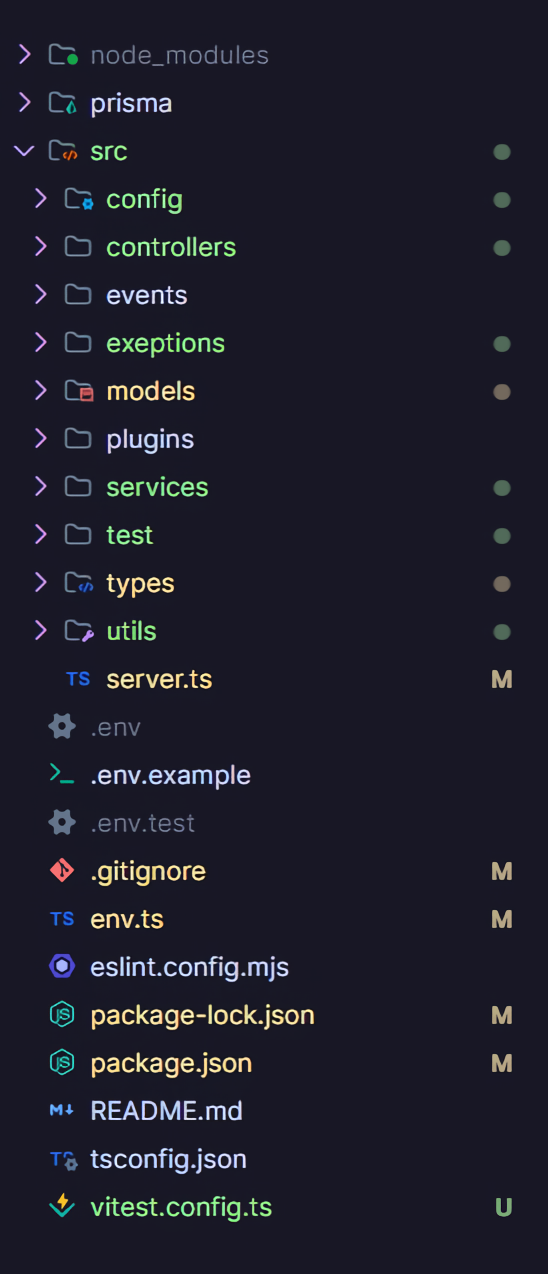
\includegraphics[scale=0.3]{img/pastas.png}
	\legend{Fonte: Autoria Própria}
	\label{fig:EstruturaDePastas}
\end{figure}


\subsection{Requisitos Funcionais}

Na sequência, foi realizado o levantamento dos requisitos técnicos, divididos em funcionais e não funcionais, com o objetivo de identificar os recursos mínimos necessários para o funcionamento inicial da aplicação, bem como visualizar,de forma mais clara, possíveis necessidades futuras, visando garantir um melhor desempenho na versão final. Nesse contexto, as funcionalidades foram definidas na tabela 6 como requisitos funcionais do sistema e, na tabela 7, como requisitos não funcionais - responsáveis por descrever as possíveis restrições do sistema até o presente momento, podendo ser implementadas futuramente.

%Tabela de levantamentos de requisitos Funcionais 
\newpage
\begin{longtblr}[,
	caption = {Tabela de Requisitos Funcionais do Sistema.},
	label = {tab:requisitos},
	]{
		width = \linewidth,
		colspec = {Q[140]Q[160]Q[680]},
		row{1} = {c},
		cell{2}{1} = {c},
		cell{2}{2} = {c},
		cell{3}{1} = {c},
		cell{3}{2} = {c},
		cell{4}{1} = {c},
		cell{4}{2} = {c},
		cell{5}{1} = {c},
		cell{5}{2} = {c},
		cell{6}{1} = {c},
		cell{6}{2} = {c},
		cell{7}{1} = {c},
		cell{7}{2} = {c},
		cell{8}{1} = {c},
		cell{8}{2} = {c},
		hlines,
		vlines,
	}
	\textbf{Referência} & \textbf{Requisito} & \textbf{Descrição}\\
	RF01 & Criação de conta & Um novo usuário poderá ser cadastrado informando um nome, e-mail e número de telefone.\\
	RF02 & Cadastro de veículo & Cadastrar um veículo é o que possibilitará ao usuário oferecer uma carona.\\
	RF03 & Reserva de carona & Os usuários podem solicitar ou oferecer uma carona. A segunda possibilidade somente será válida para aqueles com algum veículo devidamente registrado na plataforma.\\
	RF04 & Mensagens & Os interessados na carona poderão trocar mensagens entre si com o objetivo de facilitar o encontro, definir horários e decidir detalhes da viagem.\\
	RF05 & Filtrar caronas na região & Todos os usuários podem ver as caronas oferecidas na região especificada. Cada anúncio terá informações de destino, hora da viagem, lugares disponíveis e, se aplicável, o valor.\\
	RF06 & Avaliações & A avaliação ocorrerá entre motorista e passageiro, sendo uma etapa fundamental para garantir a segurança de todos os usuários. Poderá ser atribuída uma mensagem de caráter opinativo para o público e uma nota que varia de 1 a 5.\\
	RF07 & Serviços de e-mail & Envio de e-mails específicos de notificação após determinadas ações do usuário. Será possível disparar mensagens de boas vindas, criação de corrida bem sucedida, desativação e reativação de conta, entre outras.
\end{longtblr}

% Tabela requisitos não funcionais 
% \usepackage{tabularray}
\begin{longtblr}[,
	caption = {Requisitos Não Funcionais do Sistema.},
	label = {tab:requisitos},
	]{
		width = \linewidth,
		colspec = {Q[140]Q[160]Q[680]},
		row{1} = {c},
		cell{2}{1} = {c},
		cell{2}{2} = {c},
		cell{3}{1} = {c},
		cell{3}{2} = {c},
		cell{4}{1} = {c},
		cell{4}{2} = {c},
		cell{5}{1} = {c},
		cell{5}{2} = {c},
		cell{6}{1} = {c},
		cell{6}{2} = {c},
		cell{7}{1} = {c},
		cell{7}{2} = {c},
		cell{8}{1} = {c},
		cell{8}{2} = {c},
		hlines,
		vlines,
	}
	\textbf{Referência} & \textbf{Requisito} & \textbf{Descrição}\\
	RNF01 & Verificação de documentos pessoais~ & Validar se os documentos cadastrados na plataforma são válidos.\\
	RNF02 & Consulta veicular & Consultar se os dados do veículo informados pelo usuário estão cadastrados na base de dados do departamento de trânsito\\
	RNF03 & Pesquisa de antecedentes criminais & A funcionalidade poderia aumentar a segurança do usuário.\\
	RNF04 & Ranking de confiança & Os usuários com a melhor pontuação poderiam ter privilégios de divulgação ao oferecer ou solicitar uma carona.\\
	RNF05 & Pagamentos & Serviços de pagamento com o objetivo de monetizar a aplicação, além da possibilidade de motoristas lucrarem de forma justa.~\\
	RNF06 & Mensagens automatizadas & O usuário pode utilizar um recurso de inteligência artificial para gerar mensagens rápidas no chat ao solicitar ou oferecer uma carona.\\
	RNF07 & Canal de Suporte & Canal dedicado para oferecer suporte para possíveis problemas e esclarecer dúvidas frequentes.

\end{longtblr}

% INICIO Critérios de Aceitação
\subsection{Critérios de Aceitação}

Os Critérios de Aceitação são fundamentais para garantir que o software atenda aos requisitos estabelecidos e ofereça uma experiência segura e funcional aos usuários. Esta seção define as condições e requisitos que devem ser cumpridos para que a versão final do sistema seja considerada aprovada e esteja pronta para uso.

\begin{enumerate}
	
	\item \textbf{Cadastro de Usuários}
	\begin{itemize}
		\item Usuários devem se cadastrar com e-mail válido e senha forte.
		\item O e-mail deve ser único.
		\item A senha deve ter no mínimo 8 caracteres.
		\item Usuários devem fornecer informações pessoais básicas.
		
	\end{itemize}
	
	\item \textbf{Segurança}
	
	\begin{itemize}
		\item Encriptação de senha no banco de dados com um\textit{ hash}.
		\item As fotos de perfil e documentos ficarão salvos na \textit{Amazon S3}.
		\item E-mails de alerta quando dados críticos sofrerem alteração (e-mail, senha).
		\item Alterar a senha possui uma quantidade máxima de tentativas por \textit{token}.
	\end{itemize}
	
	\item \textbf{Perfil de Usuário}
	
	\begin{itemize}
		\item Usuários podem atualizar seu perfil a qualquer momento.
		\item Possibilidade de alterar nome, telefone, foto de perfil, etc.
		\item Endereço de e-mail e data de nascimento não podem ser alterados sem verificação adicional.
		\item Usuários devem verificar seu e-mail após o cadastro.
		\item Envio de um e-mail de confirmação com um link para ativar a conta.
	\end{itemize}
	
	\item \textbf{Cadastro de Veículos}
	
	\begin{itemize}
		\item Motoristas devem cadastrar seus veículos para oferecer caronas.
		\item Informar marca, modelo, ano, placa, cor e número de assentos disponíveis.
		\item Motoristas devem enviar documentos comprobatórios relativos ao veículo.
	\end{itemize}
	
	\item \textbf{Publicação de Viagens}
	
	\begin{itemize}
		\item Motoristas podem criar viagens detalhando rota, data, hora e pontos de embarque/desembarque.
		\item Especificar preço por passageiro, se aplicável.
		\item Informar restrições ou preferências dos envolvidos na viagem.
		\item As viagens devem ser criadas com antecedência mínima.
		\item Definir um tempo mínimo antes do horário de partida para criação de novas viagens.
	\end{itemize}
	
	\item \textbf{Reserva de Caronas}
	
	\begin{itemize}
		\item Passageiros podem reservar vagas nas viagens disponíveis.
		\item Confirmar a reserva mediante pagamento, se aplicável.
		\item Notificação para motorista e passageiro sobre a reserva confirmada.
		\item Passageiros podem cancelar suas reservas.
		\item Definir, quando aplicável, políticas de cancelamento e reembolso.
	\end{itemize}
	
	\item \textbf{Avaliação e Feedback}
	
	\begin{itemize}
		\item Usuários podem avaliar e deixar feedback sobre as viagens.
		\item Motoristas e passageiros podem se avaliar mutuamente.
		\item Avaliações devem ser visíveis nos perfis dos usuários.
	\end{itemize}
	
	\item \textbf{Suporte}
	
	\begin{itemize}
		\item Monitoramento e resolução de problemas.
		\item Canal de suporte ao usuário para resolução de problemas e disputas.
	\end{itemize}

\end{enumerate}

% FIM dos critérios de Aceitação

% FIM Arquitetura 

\section{Tecnologias e Ferramentas}

O desenvolvimento de software exige uma variedade de recursos durante a produção. Escolher cuidadosamente as ferramentas a serem utilizadas no ambiente de desenvolvimento garante a qualidade, funcionalidade, eficácia, escalabilidade e eficiência do sistema. Nesse contexto, as seguintes tecnologias foram empregadas durante o desenvolvimento: 

\subsection{Ambiente de Trabalho}

\begin{enumerate}
	\item\textit{ Visual Studio Code} - editor de código-fonte gratuito que permite a integração com \textit{Git}, facilitando \textit{commits, pushes, pulls e merges}, além de possibilitar o uso do \textit{intelliSense} para melhorar a produtividade no ambiente de trabalho.
	
	\item \textit{GitHub} -  plataforma de hospedagem de código-fonte que permite o versionamento \textit{ Git}. Foi de suma importância para que cada colaborador trabalhasse na implementação das mudanças nos repositórios da organização.
	
	\item \textit{Node.js} -  Ferramenta de execução e interpretação da linguagem \textit{JavaScript} que permite o seu uso no ambiente de desenvolvimento, sendo de suma importância para executar os códigos criados ao lado do servidor com tal linguagem. 
\end{enumerate}


\subsection{Linguagem de Programação}

\begin{enumerate}
	\item \textit{JavaScript} -   linguagem de programação escolhida devido a sua  versatilidade, facilidade de uso, sintaxe limpa e grande oferta de \textit{frameworks.}
	\item \textit{TypeScript} - é o superset do \textit{JavaScript} que adiciona tipagem estática à linguagem,  permitindo com que o desenvolvedor possa definir os tipos de dados das suas variáveis, funções e objetos com a finalidade de tornar o código mais seguro, previsível e escalável, além de facilitar futuras refatorações

\end{enumerate}

\subsection{\textit{Framework}}
\textit{Fastify} - Uma das melhores opções entre os frameworks para \textit{Node.js,} sendo rápido, flexível e com uma excelente experiência de desenvolvimento. Foi fundamental para construir aplicações web escaláveis e de alto desempenho, além de oferecer uma boa integração com o \textit{TypeScript.}

\subsection{Banco de Dados}

\begin{enumerate}

	\item \textit{Prisma - ORM (Object-Relational Mapper)} escolhido para as interações com o banco de dados, sendo fundamental para criar migrações, assim criar, ler, atualizar e deletar dados no banco de dados se tornou mais rápido e com menos código, reduzindo a possibilidade de erros.
	
	\item  \textit{MySQL} - SGBD (Sistema Gerenciador de Banco de Dados) responsável por armazenar, organizar e gerenciar dados. É conhecido pela confiabilidade e ampla utilização nos mais variados ambientes de desenvolvimento.
	
	\item BrModelo -  foi uma ferramenta importante na modelagem do banco de dados, permitindo a elaboração de diagramas entidade-relacionamento (ER) e facilitando a sua visualização antes da implementação da versão final do banco.
	
\end{enumerate}

\subsection{Produtividade}

\begin{enumerate}
	
	\item \textit{Trello} - Utilizado para o gerenciamento do projetos baseado em metodologia visual, por meio de um sistema de quadro de Kanban, dividindo uma tarefa em várias ações para que todos os integrantes do grupo participem do projeto de forma coesa.
	
	%\begin{figure} [h!]
		%\centering
		%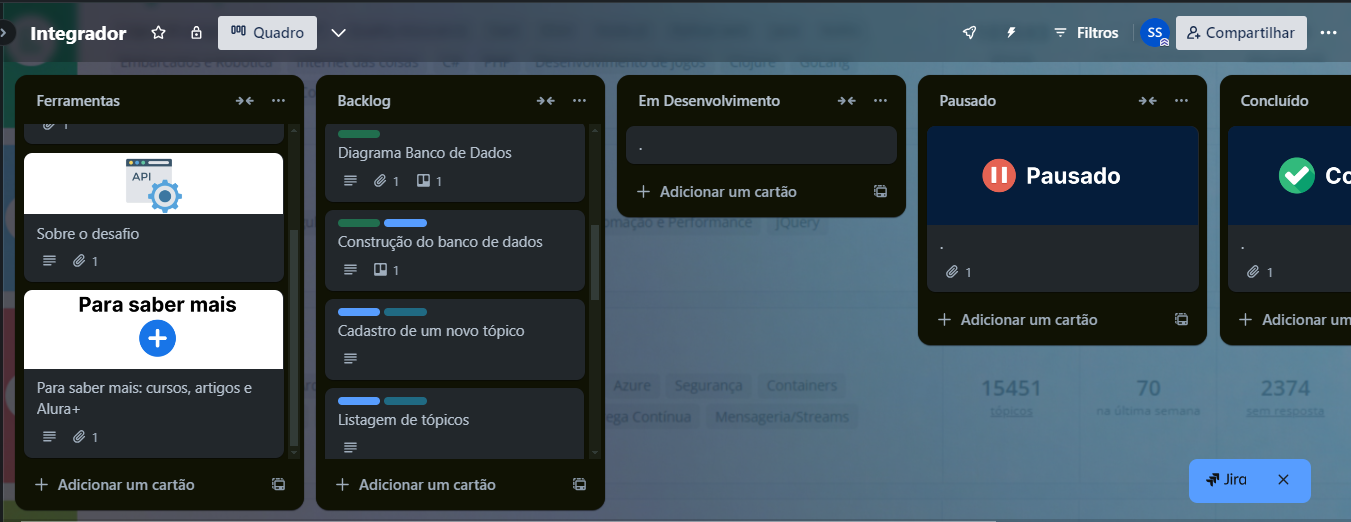
\includegraphics[scale=0.4]{img/trello.png}
		%\caption{Trello da Equipe,2024}
		%\label{fig:Produtividade}
	%\end{figure}
	
	
	\item \textit{ Notion} -  Necessário para os desenvolvedores centralizarem as informações importantes, bem como anotações desenvolvidas ao longo do trabalho. Entre as suas vantagens destaca-se a facilidade de uso e a integração com outras ferramentas.
	
\end{enumerate}



% ---
% Conclusão
% ---
\chapter{Considerações finais}
% ---

Faça um breve resumo do tema e dos objetivos propostos para o trabalho. Em seguida, recapitule os principais resultados obtidos durante o desenvolvimento do sistema, apontando os marcos positivos e negativos que ocorreram durante o processo.

Para finalizar o capítulo, descreva as limitações de sua solução e apresente propostas de melhorias futuras para o sistema.

--------------

Para ajudá-los a fazer citações de artigos, livros, sites e demais fontes de informação em LaTeX, deixarei esse pequeno parágrafo. Basicamente, há três formas de citar um material: 1) comando \textbf{cite}; 2) comando \textbf{citeonline}; e 3) o bloco \textbf{citacao}. 

O comando \textbf{cite} apresenta o seguinte formato no PDF: \cite[p. 23]{abntex2-wiki-como-customizar}. O comando \textbf{cite} é usado quando se faz uma \textbf{citação direta curta}, após colocar-se o texto retirado da fonte entre as aspas.

Já o comando \textbf{citeonline} apresenta o seguinte formato no PDF: \citeonline{abntex2-wiki-como-customizar}. Esse comando é usado quando se faz uma \textbf{citação indireta}, que é aquela onde se replica a \textbf{ideia do autor, mas as palavras são suas}. Esse tipo de formato de citação costuma aparecer ``entre o texto'', não no final.

Por fim, o bloco citacao é utilizado para citações diretas que possuem mais de 3 linhas. Elas têm formatação diferente conforme as regras da \citeonline{NBR6024:2012}.

\begin{citacao}
    Esta é uma \textbf{citação direta longa}, ou seja, é uma citação que possui mais de 3 linhas copiadas literalmente de alguma fonte de informação utilizada no trabalho. Observe que o bloco \textbf{citacao} é usado em conjunto com o comando \textbf{cite}. \cite[p. 11]{abntex2-wiki-como-customizar}.
\end{citacao}


% ----------------------------------------------------------
% ELEMENTOS PÓS-TEXTUAIS
% ----------------------------------------------------------
\postextual

% ----------------------------------------------------------
% Referências bibliográficas
% ----------------------------------------------------------
\bibliography{referencias}


% ----------------------------------------------------------
% Anexos
% ----------------------------------------------------------

% ---
% Inicia os anexos
% ---
\begin{anexosenv}

% ---
\chapter{MODELO ENTIDADE-RELACIONAMENTO (MER)}
% ---
\begin{figure}[h!]
	\centering
	\rotatebox{270}{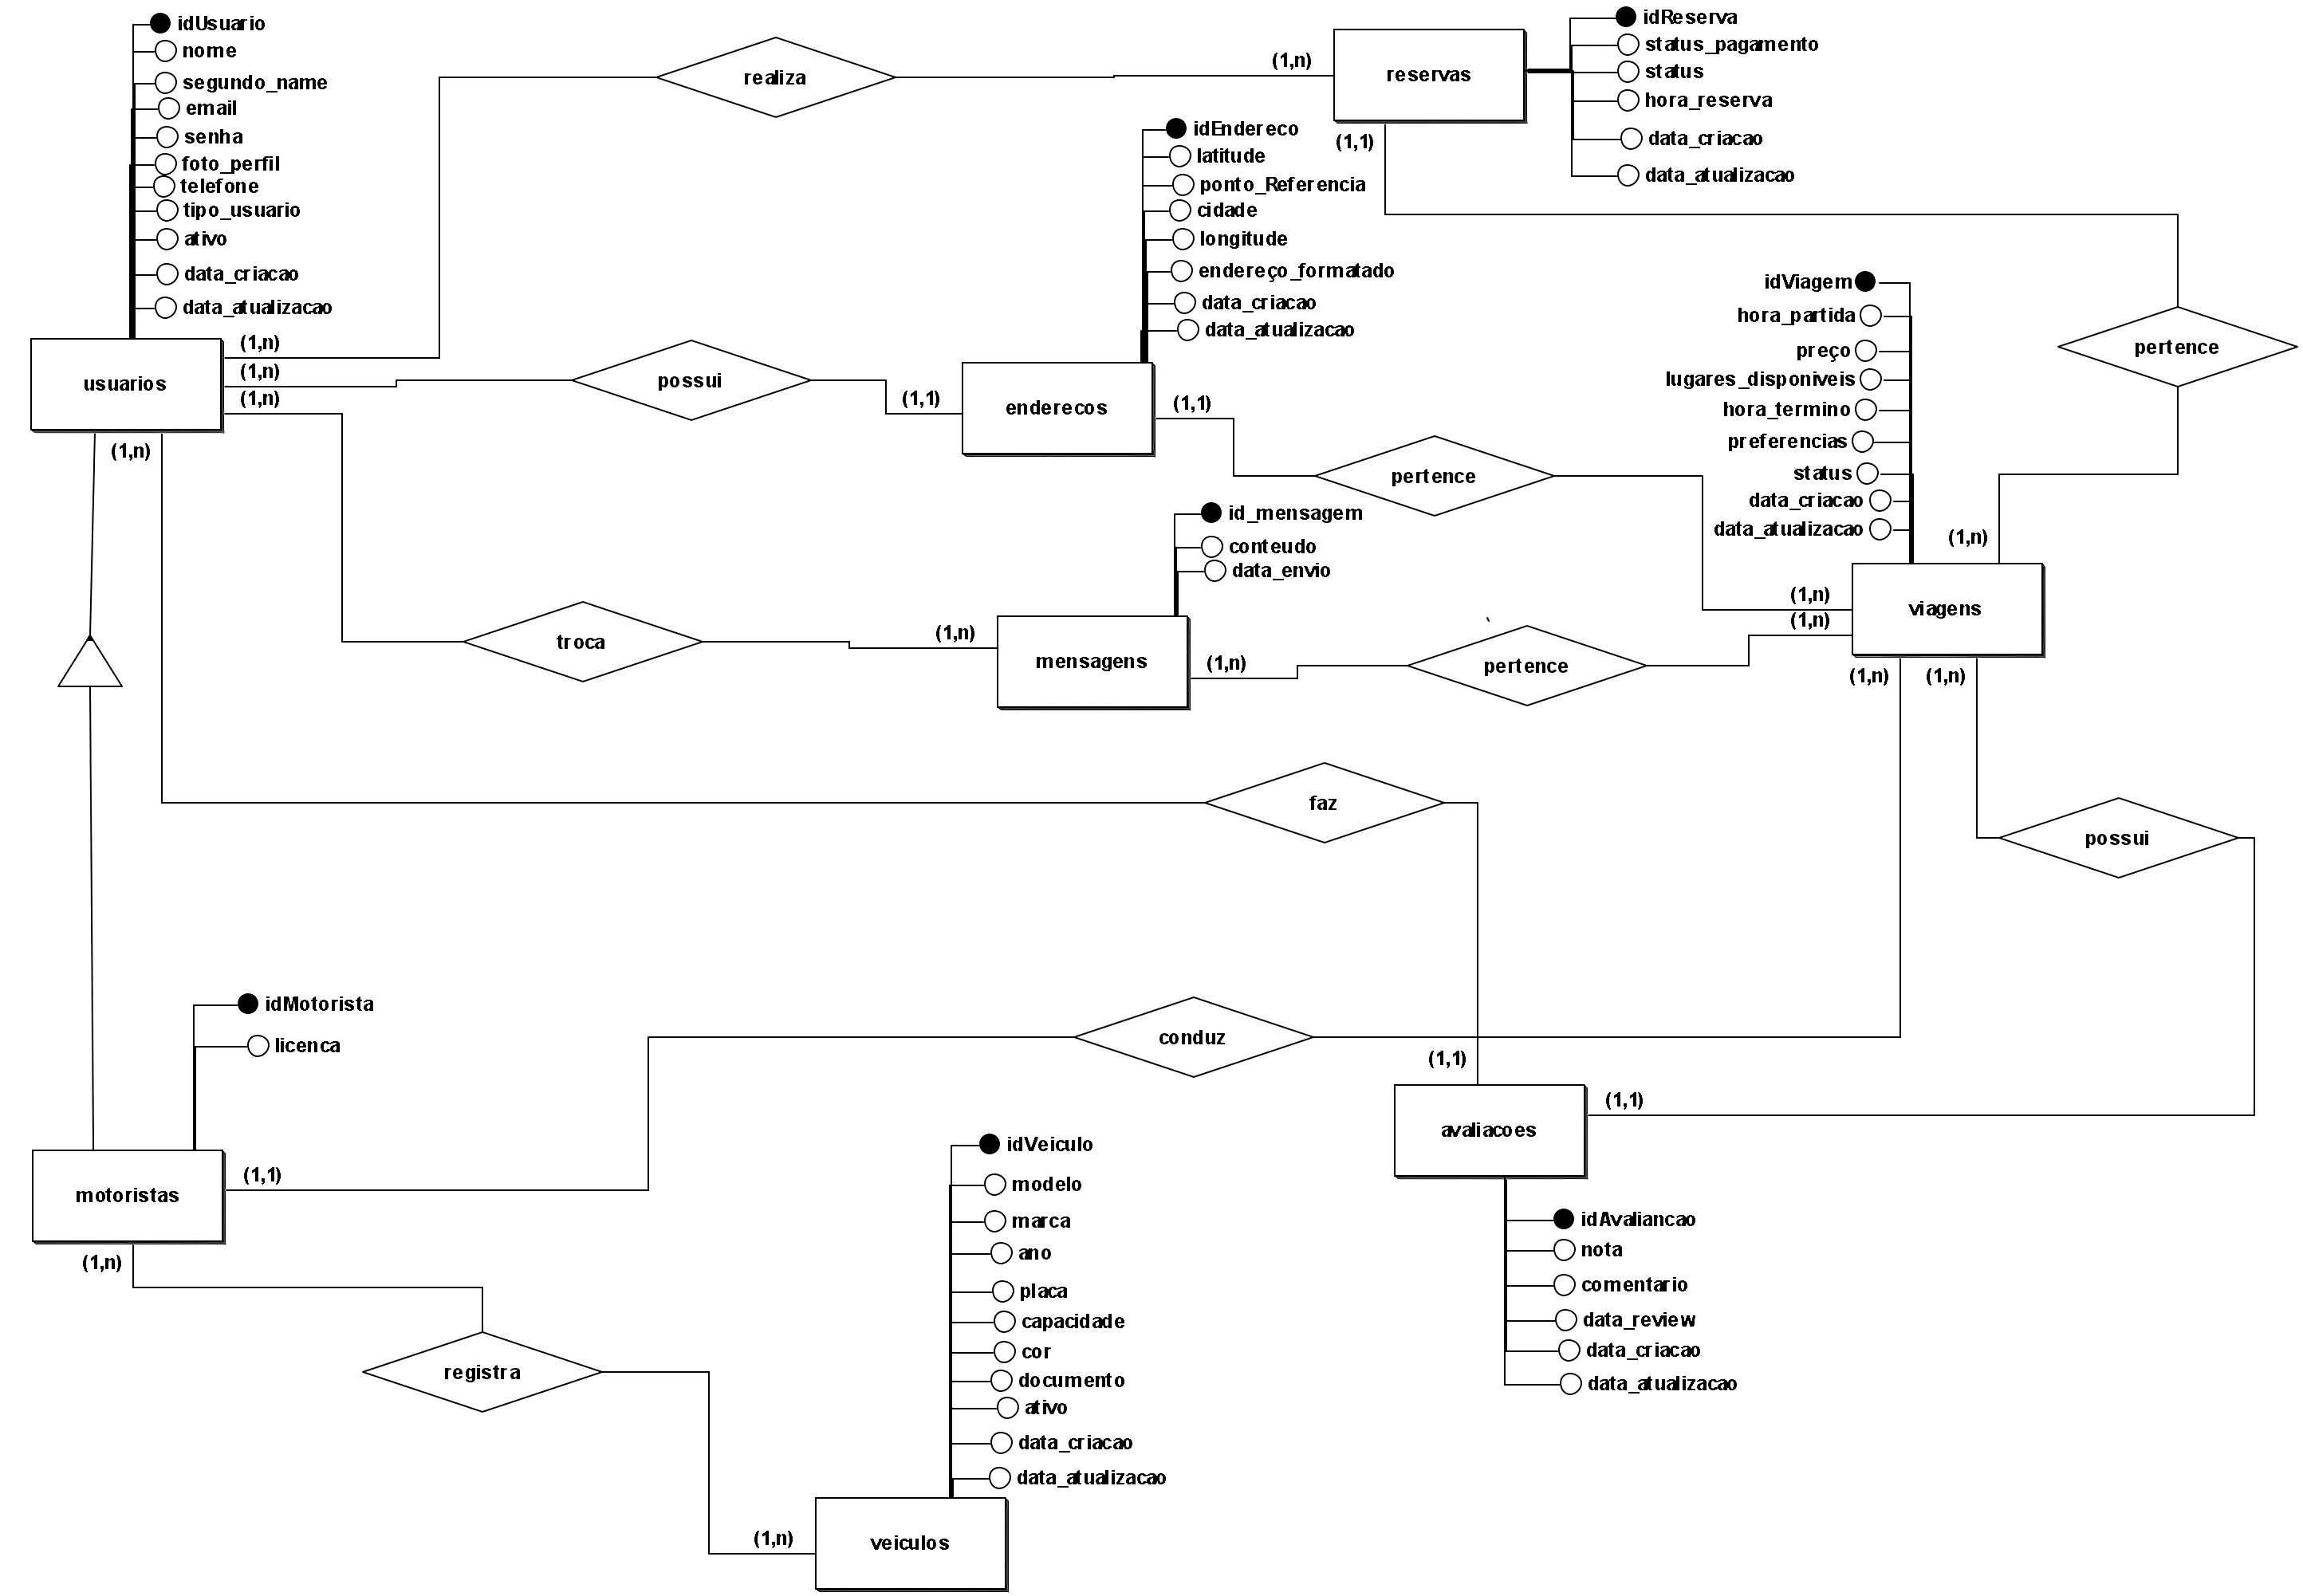
\includegraphics[width=1.24\textwidth]{img/AnexoA.png}}
	%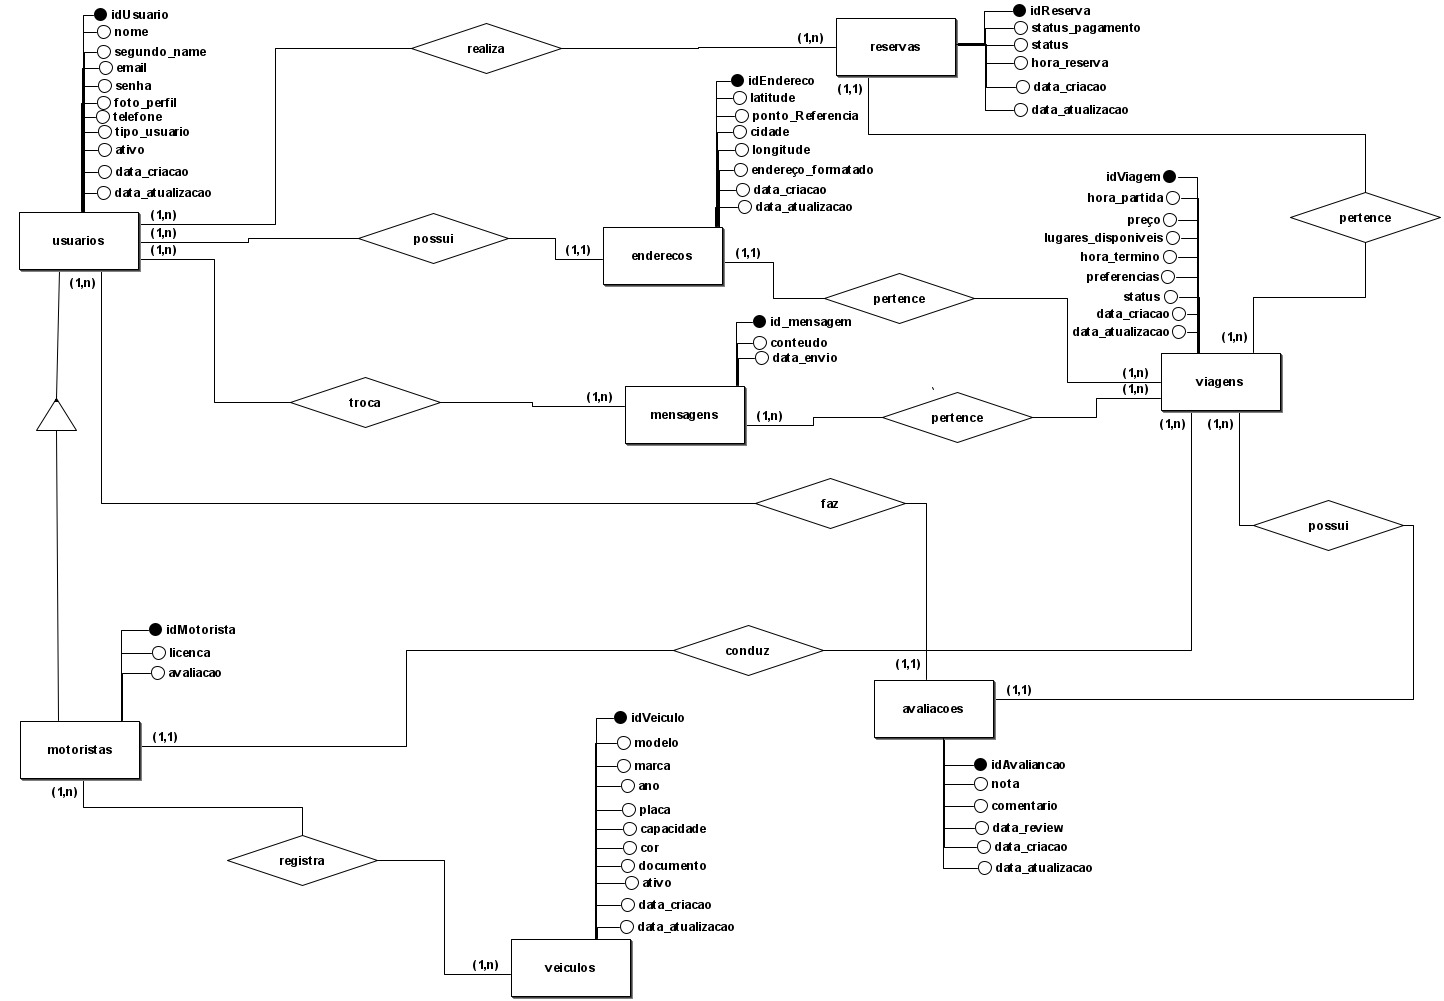
\includegraphics[width=1\linewidth]{img/AnexoA.jpg}
	\caption{Modelo Conceitual - Aplicativo de Caronas}
	\label{fig:modelo_conceitual_banco}
\end{figure}


% ---
\chapter{DIAGRAMA ENTIDADE-RELACIONAMENTO (DER)}
% ---

\begin{figure}[h!]
	\centering
	\rotatebox{270}{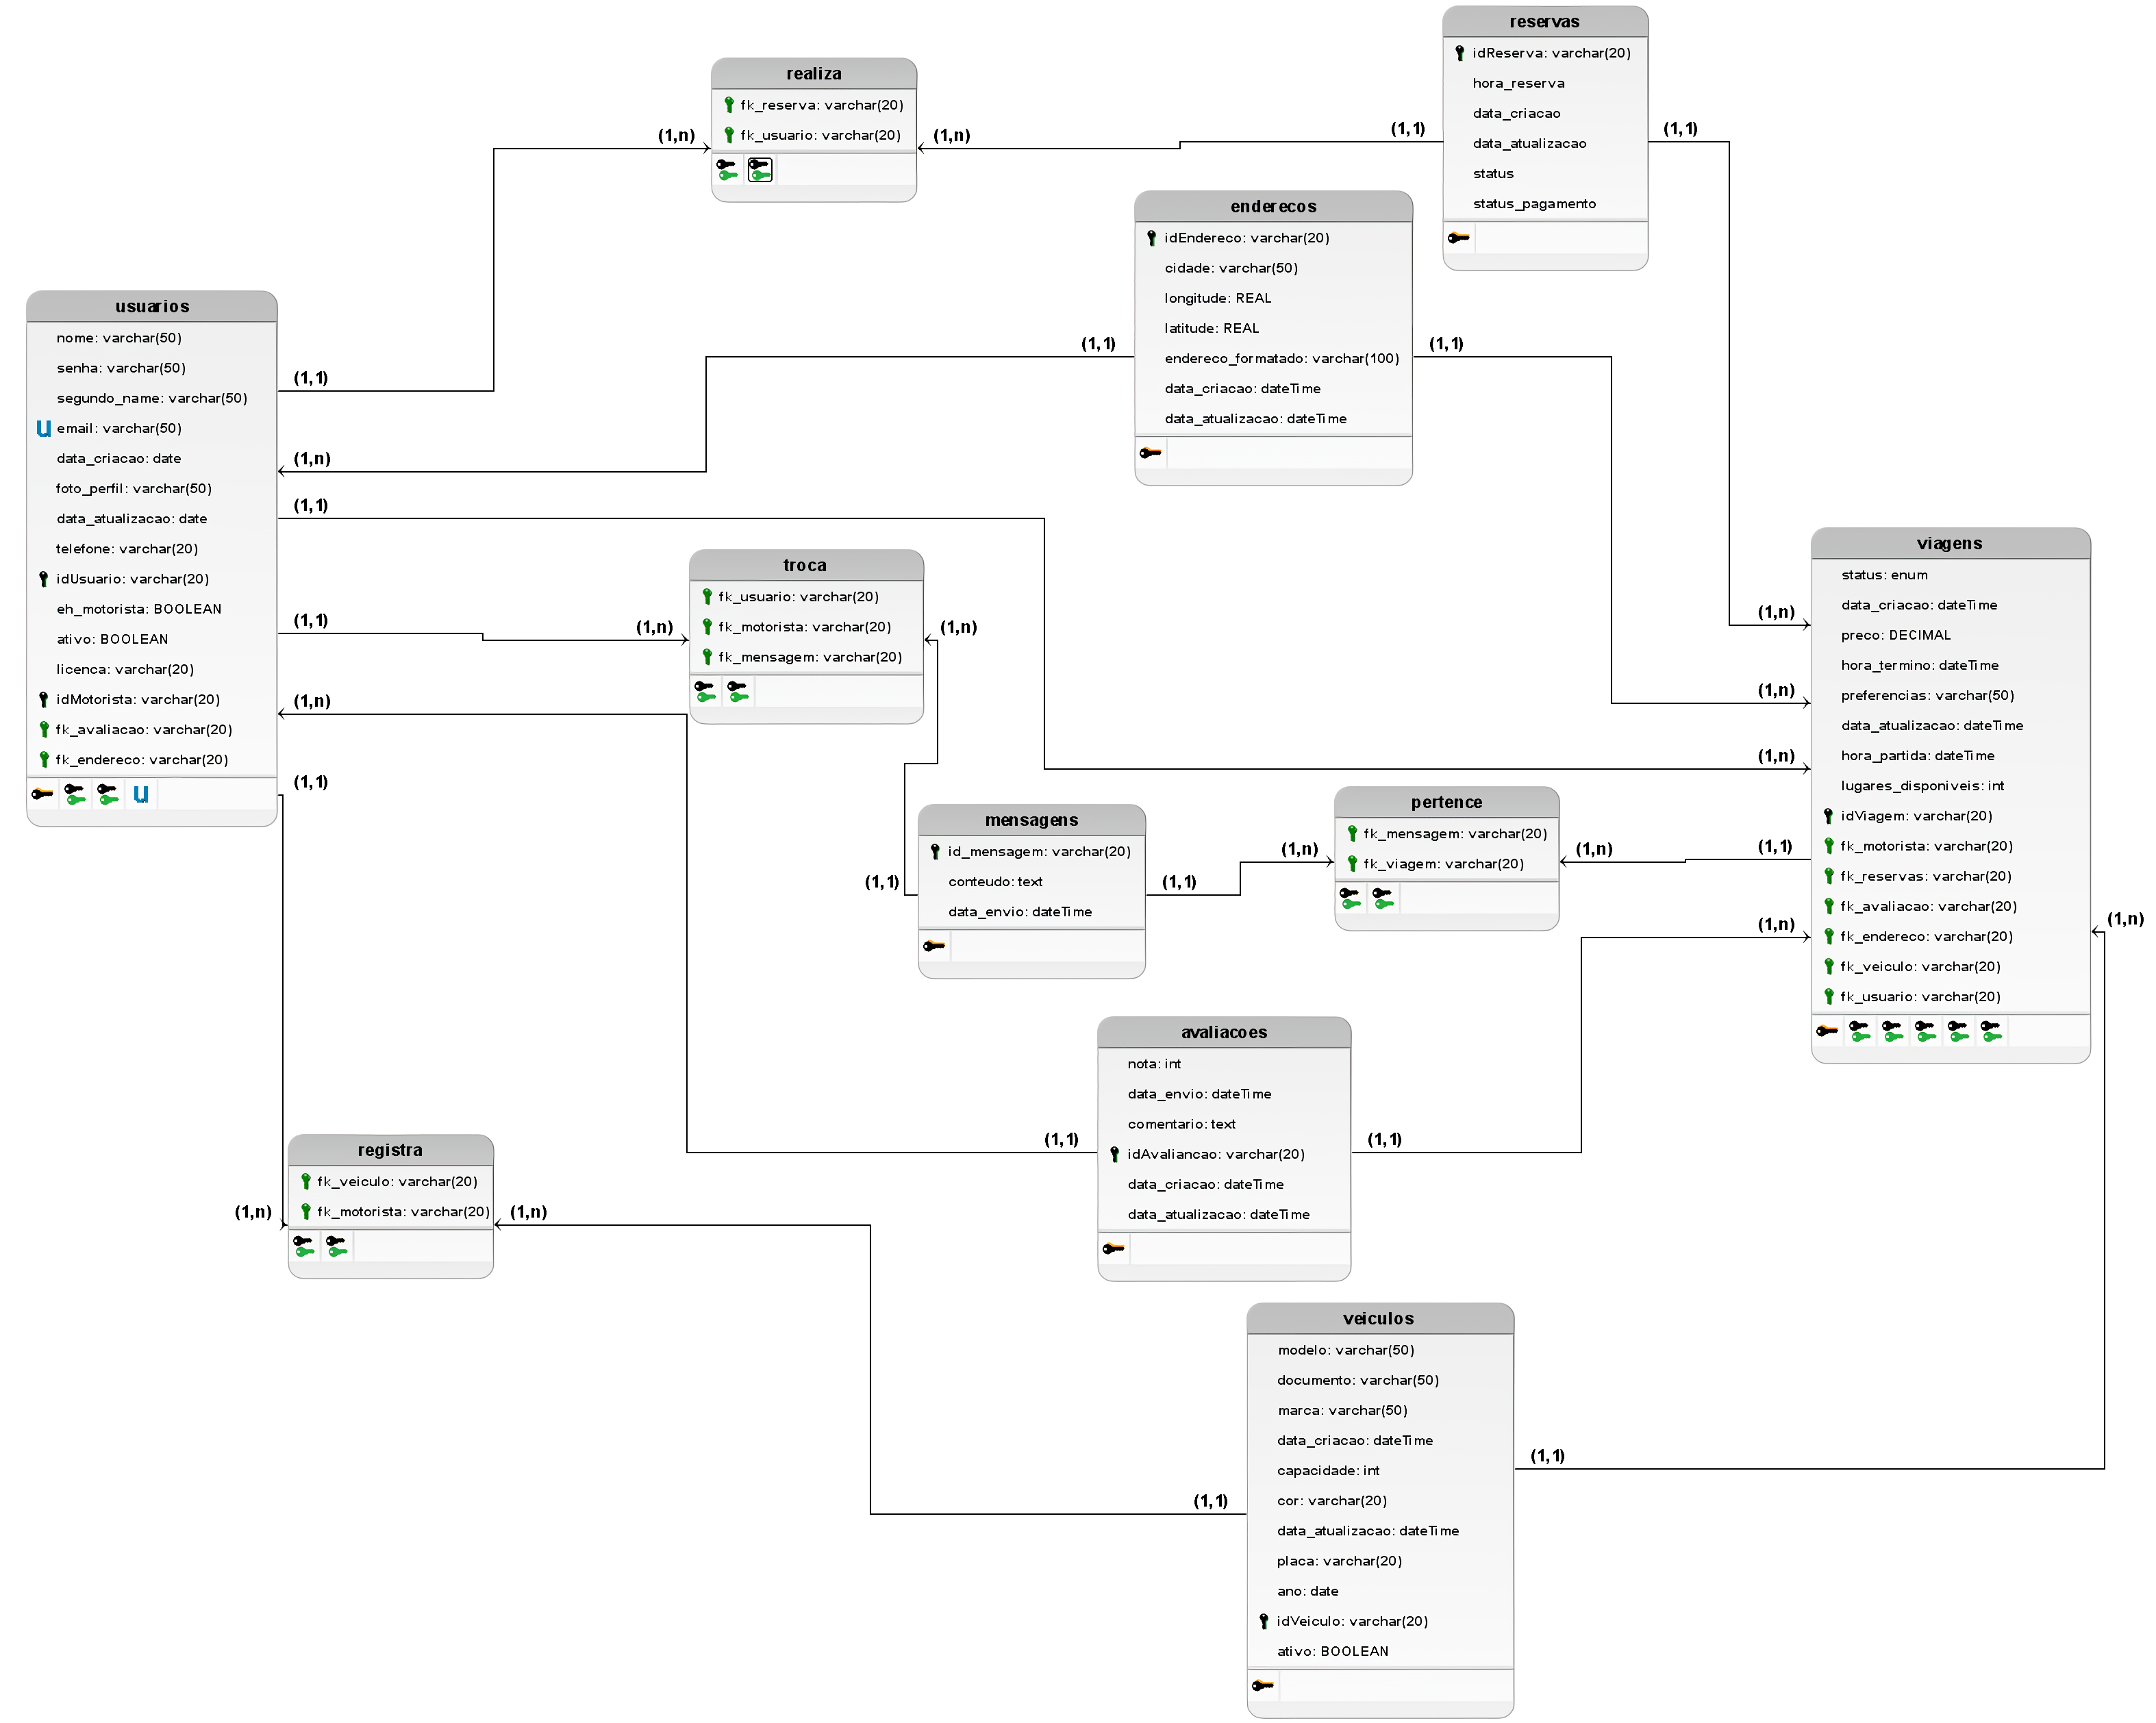
\includegraphics[width=1.24\textwidth]{img/AnexoB.png}}
	%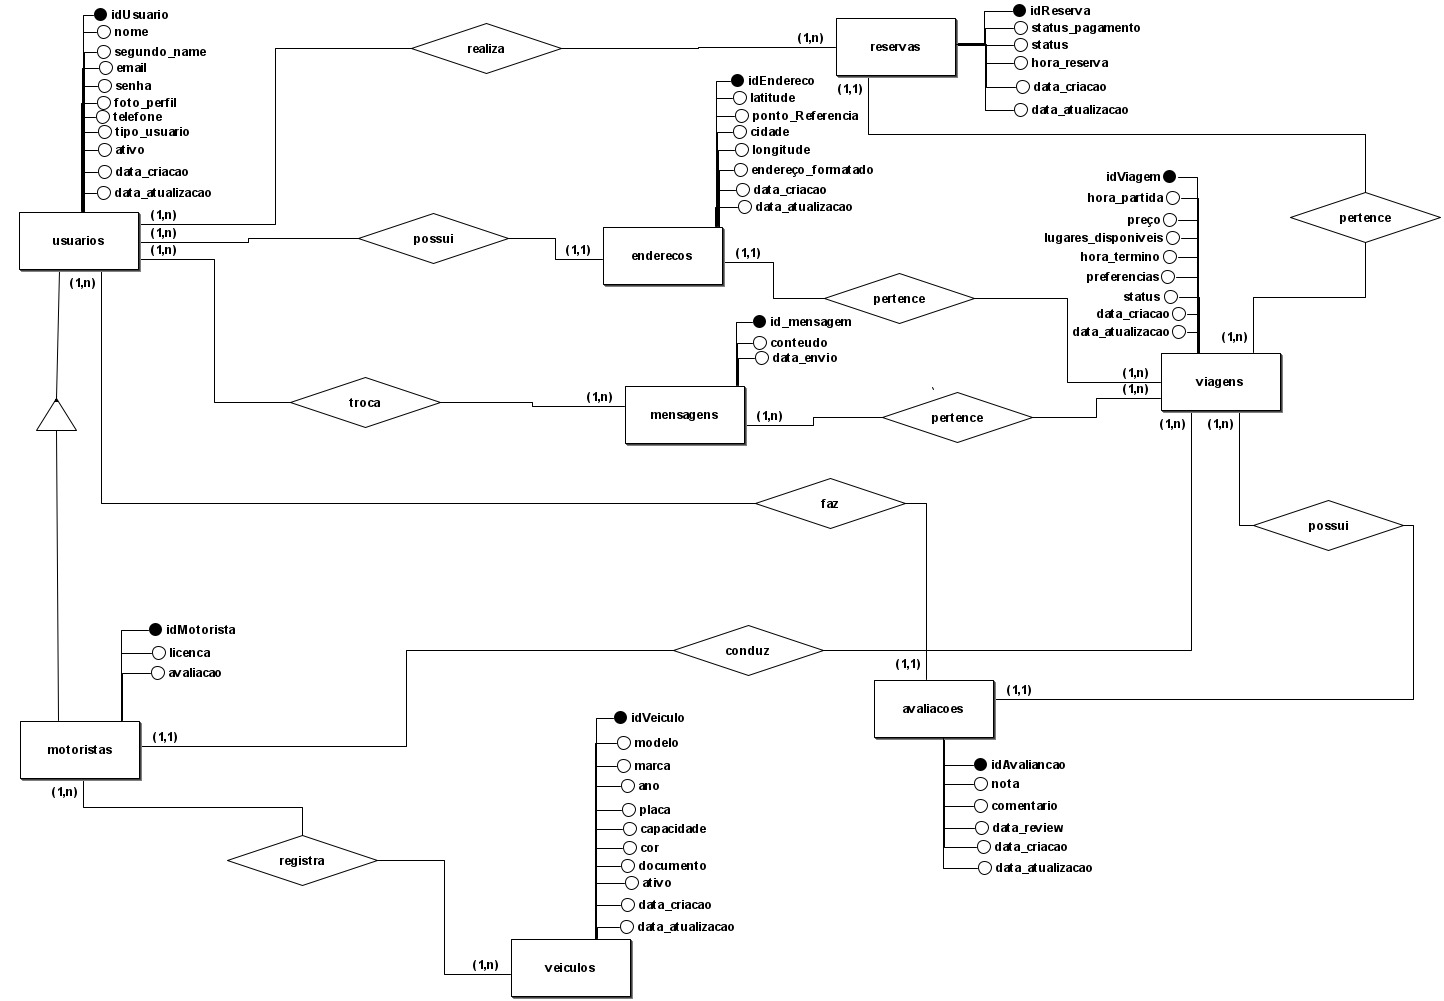
\includegraphics[width=1\linewidth]{img/AnexoA.jpg}
	\caption{Modelo Lógico- Aplicativo de Caronas}
	\label{fig:modelo_logico_banco}
\end{figure}


% ---
%\chapter{Título do anexo C}
%Coloque o conteúdo do seu anexo aqui (se houver).

\end{anexosenv}


\printindex

%----
% Define tabela 

%----

\end{document}
